\documentclass[11pt]{article}
\usepackage{common}
\usepackage[usenames, dvipsnames]{color}
\usepackage{setspace}
\usepackage{booktabs}
\usepackage{multirow}

\title{Exploring Optimization Strategies for \textit{Mastermind}}
\author{Gioia Domined\`o \and Amy Lee \and Kendrick Lo \and Reinier Maat}

\begin{document}
\maketitle{}

\begin{abstract}
\noindent We implement variations on five iterative ``code-breaking" optimization methods for solving the classic game \textit{Mastermind}. We test our techniques on 14 different game board configurations of varying complexity and report empirical performance in terms of the average number of guesses required to win the game, and the average computational time for playing all turns of the game. We find that global optimization methods are able to consistently win the game in a small number of moves but require excessive runtimes for even moderately complex game board configurations. Local optimization methods require more moves to win the game, but are able to approximate ``real time" game playing even on the more complex game boards.
\end{abstract}

\pagestyle{plain}
\pagenumbering{arabic}

\section{Introduction}

The game \textit{Mastermind} was invented in 1970 by Mordecai Meirowitz, and is similar to an earlier game called Bulls and Cows. There are many variations of the game, but they all follow a broadly consistent format. The game involves two players: a code-maker and a code-breaker. The code-maker selects a sequence of length L (usually 4), where each element in the sequence is chosen with replacement from one of C colors (usually 6). At each turn, the code-breaker guesses a sequence and receives feedback in the form of black pegs and white pegs, where the black pegs denote the number of correct guesses in the right position, and the white pegs denote the number of correct guesses in the wrong position. Based on this information, the code-breaker refines her guesses and attempts to crack the code within the maximum number of guesses (usually 10).

For our project, we set out to implement various strategies and algorithms for iteratively optimizing the code-breaker's guess at each turn. We compared the performance of these strategies based on the mean and standard deviation of the required number of guesses to win and the runtime across 20 random game initializations. In order to assess the extent to which the different solutions scale efficiently, we tested 14 game board configurations of varying complexity.

\begin{figure}[!htbp]
\centering
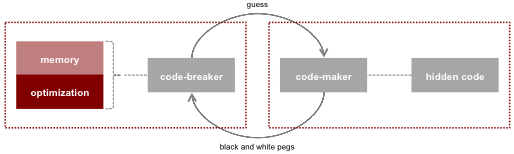
\includegraphics[width=0.59\textwidth]{img/game_setup}
\caption{Mastermind Framework}
\label{fig:game_setup}
\end{figure}

\newpage

\section{Optimization Methods}

We began the project by developing a Python implementation of \textit{Mastermind}, which we used to test multiple code-breaking optimization methods on boards of varying complexity. Before describing the methods, it is helpful to frame the game in some mathematical notation, which we will also use in the descriptions of the methods below. For simplicity, we use one-indexing in all formulas; however, we note that the Python code for the game interface is zero-indexed.

We define the set of colors as $CC = \{1, ..., C\}$, and the set of code positions as $LL = \{1, ..., L\}$. Each item of the $L$-length code is denoted as  $H_i$, and each item of a given $L$-length guess is denoted as $T_i$. For convenience, we also define the indicator function $\mathbb{1}_{A=B}$, which equals $1$ if $A=B$ and $0$ otherwise. Using this notation, we can denote the response tuple at each turn as $(B, W)$, where $B$ and $W$ represent the number of correct guesses in the right position, and the number of correct guesses in the wrong position, respectively. We calculate these as $B= \sum_{i=1}^L \mathbb{1}_{T_i=H_i} \ \forall i \in L$ and $W = \sum_{i=1}^{C} \min(\sum_{j=1}^{L}\mathbb{1}_{H_j=i, G_i}, \sum_{j=1}^{L}\mathbb{1}_{T_j=i, G_i}) - B$.

\subsection{Knuth's Five-Guess Algorithm}

The most commonly referenced optimization technique in the \textit{Mastermind} literature is Knuth's five-guess algorithm \cite{knuth76} \textendash \ sometimes also referred to as the ``worst-case strategy" \textendash \ which can always solve the classic game configuration in five moves or less. This strategy always begins with the same initial guess of 1122 (or 0011, when zero-indexed); this choice is motivated by examples of other initial guesses that do not always lead to a solution in five moves. Our implementation uses this deterministic initial guess for the classic game configuration, but uses a random initial guess for all other configurations, as analogous ``best" starting points are not defined in the literature.

After the initial guess, the algorithm determines the minimum number of codes that each guess would eliminate from the list of possibilities, and chooses one of the guesses that maximizes this number\footnote{Wikipedia refers to this as the minimax \textit{technique}. We note that this one-off maximization differs from the recursive minimax \textit{algorithm} that is also used in game theory.}. At each stage of the game, the set of possible codes is updated to only include codes that would have generated the same responses at all of the previous steps. This ensures that the search space of possible guesses shrinks at each turn.

\subsection{Random Search with Constraints / Random Sampling From Posterior}

This method is described in the \textit{Mastermind} literature both as a constrained random search algorithm \cite{bernier1996solving} and in terms of posterior distribution updates \cite{vomlel2004bayesian}. We follow the latter approach, and start by defining the joint probability distribution over all possible code sequences as $P(H_1, ..., H_L)$. As we have no information, our prior is uniformly distributed.

\[
P(H_1=h_1, ..., H_L=h_l) = \frac{1}{C^L} ,\quad \text{for all combinations of }(h_1, ..., h_l)
\]

\noindent We can denote the evidence that is obtained at each step as $e = (B, W)$, where B and W are defined as above, and use this to update the posterior joint distribution over code sequences as follows:

\[
    P(H_1=h_1, ..., H_L=h_l | e) = 
\begin{cases}
    \frac{1}{|s(e)|},& \text{if } (h_1, ..., h_l) \ \text{is a possible code}\\
    0,              & \text{otherwise}
\end{cases}
\]

\noindent where s(e) denotes the set of possible hidden codes, given the evidence, and $|s(e)|$ denotes the cardinality of this set. \medskip

\noindent We can define the posterior after multiple game steps analogously:

\[
    P(H_1=h_1, ..., H_L=h_l | e_1, ..., e_n) = 
\begin{cases}
    \frac{1}{| s(e_1) \ \cap \ ... \ \cap \ s(e_n) |},& \text{if } (h_1, ..., h_l) \ \text{is a possible code}\\
    0,              & \text{otherwise}
\end{cases}
\]

\noindent where $\ s(e_1) \ \cap \ ... \ \cap \ s(e_n)$ denotes the intersection of the sets of possible hidden codes, given the evidence at each step, and the entire denominator denotes the cardinality of this intersection.

We can use this framework to define the posterior updates at each round of the game, and then choose the next guess by sampling from the posterior distribution. Figure \ref{fig:num_guesses} shows how the number of possible guesses shrinks as the game progresses.

\subsection{Maximizing Shannon Entropy}

Entropy is a measure that is commonly used in information theory to quantify the average amount of information that is contained in a message. In the context of \textit{Mastermind}, the ``message" is the response of black and white pins that is returned by the code-maker at each turn. The goal of the code-breaker is to choose guesses that create as even a distribution as possible between the various responses, as it will allow her to discard more possible codes at the next step.

Let us denote $r_i$ as the $i$th response category and R as the number of possible responses\footnote{For example, the classic version of the game with codes of length $4$ has 14 possible responses: $(4, 0), (3, 0), (2, 2), (2, 1), (2, 0), (1, 3), (1, 2), (1, 1), (1, 0), (0, 4), (0, 3), (0, 2), (0, 1), (0, 0)$.}. We can then define the entropy of the discrete response space $\{r_1, ... , r_R\}$ for a given guess as:

\[
H(\text{guess} | \text{possible codes}) = \sum_{i=1}^R P(r_i) I(r_i) = - \sum_{i=1}^R P(r_i) \log_bP(r_i)
\]

\noindent where $I(r_i)$ denotes the information content of the $i$th response category. We use $b=2$, meaning that we are measuring entropy in shannons, but note that any other value of $b$ would yield a consistent ranking between guesses.

Practically, we calculate the probability of each response category for a given guess by counting (and normalizing) the total number of possible responses in each category, given the hidden codes that are still possible at that particular stage in the game. The value will depend on the shape of the probability distribution across the response categories, with the minimum entropy of $0$ only achievable when there is certainty of a particular outcome (i.e. $log_2(1)=0$).

In order to improve her performance, the code-breaker will want to pick the guess that results in the highest entropy \textendash \ or, if there are ties, one of the best guesses \textendash \ in order to be able to discard as many codes as possible at the next step. This can be achieved through an exhaustive calculation of the entropy of all possible guesses at each stage or, for larger search spaces, through local search techniques such as simulated annealing or genetic algorithms.  Figure \ref{fig:entropy} illustrates how the distribution of entropy for the remaining possible guesses can change as the game progresses; this technique is particularly effective where there is a clear maximum value (e.g. at the third guess, in the particular game shown in the Figure).

\newpage

\subsection{Simulated Annealing}

Simulated annealing (SA) is a local optimization method that can be a powerful tool in larger search spaces\footnote{The classical SA formulation involves the minimization of a cost function. Potential solutions are proposed iteratively, and their cost is compared to that of previously accepted solutions. Solutions with lower cost are automatically accepted, while solutions with greater cost are accepted with a certain probability. This probability decreases as the ``temperature" model parameter decreases, and varies inversely with the difference between the cost of the previously accepted solution and the cost of the newly proposed solution. In practice, SA can also be used to maximize objective functions, in addition to strictly minimizing cost functions.}. The effectiveness of this technique depends upon the objective function that is used to evaluate potential guesses, and the method that is used to propose potential new guesses. As mentioned above, one application of simulated annealing is as an alternative to the global maximization of entropy across all possible guesses. In this framework, new guesses are proposed by randomly picking from the set of remaining possible guesses, and are evaluated by calculating their entropy.

We also implemented an alternative SA approach that was developed by Bernier et al. \cite{bernier1996solving}. Under this framework, new guesses are generated by introducing \textit{permutations} (swaps of code element pairs) and/or \textit{mutations} (changes to individual code elements) to the last code that was considered. The number of permutations and mutations is determined by the SA ``temperature": the code can change significantly when the temperature is high, encouraging wide exploration of the search space, but will only change slightly when the temperature is lower (by which point the code-breaker hopes to be close to the correct code), encouraging convergence to a ``good" solution.

In order to determine whether the proposed code is ``better" than the current code, we use an objective function based on the difference between the black and white pegs obtained from all previous guesses and the number of black and white pegs that would have been obtained if the newly proposed guess were the right code. The cost function is defined as:

\[
\sum_{i=1}^n | \Delta n_w^i | + | \Delta n_w^i + \Delta n_b^i |
\]

\noindent where $n$ is the number of previous guesses made and $\Delta n_w^i $ and $\Delta n_b^i$ are the differences in white and black peg responses, respectively. If the cost function evaluates to zero (i.e. the proposed guess is consistent with all the responses received until that point in the game), then the proposal is accepted as it may be the correct answer. If, instead, the proposed guess is only consistent with some of the previous responses, then it is accepted with a certain probability; while it cannot possibly be the correct solution, it may nonetheless lead the code-breaker closer to the correct solution. In this manner, SA can approach a close-to-optimal solution relatively quickly, as each evaluation of the cost function only requires a comparison to previous guesses, as opposed to the entire search space of possible guesses.

\subsection{Genetic Algorithms}

Another local optimization method is genetic algorithms (GA), which draws inspiration from natural evolution to solve optimization problems. In the context of \textit{Mastermind}, we created a population of 60 candidate guesses and evolved them toward better solutions over the course of 100 ``generations". The most eligible guesses were selected at each generation based on their ``fitness" function: we tested the same Bernier and entropy objective functions that we used for SA.

\newpage

In order to maintain diversity as across generations and efficiently explore the search space, we applied four types of alterations: \textit{crossovers between two codes}, where each position in the first code has a 0.5 probability of being crossed with the corresponding position in the second code; \textit{mutations}, where the color of a randomly chosen position is replaced by a random other color with 0.03 probability; \textit{permutations}, where the colors of two random positions have a 0.03 probability of being switched; and \textit{inversions}, where the sequence of colors between two randomly chosen positions are inverted with a 0.02 probability.

\section{Experiments}

We used two different setups to test our optimization methods: we varied the number of possible colors ($C$) between $4-10$, while maintaining the code length constant at $4$; and we varied the number of positions ($L$) between $4-10$, while keeping the number of colors constant at $2$. We played the game $20$ times with each configuration and each code-breaking optimization method, and measured the average number of guesses and runtime. Detailed results are presented graphically and in tabular form in Appendices \ref{graphical_results} and \ref{tabular_results}, and the entire code base is available online\footnote{https://github.com/dominedo/am207project}.

\paragraph{Global optimization.} The optimization methods that rely on an exhaustive search over all possible guesses performed very well in terms of actual game performance, and were able to consistently guess the right code with few moves, even in the more complex game setups. However, this came at the expense of significant runtimes; in fact, we had to redefine our planned experiments as these methods require several hours per guess on complex game board configurations!

Faced with these initial results, we experimented with variations in our implementations \textendash \ which were initially based on the classical formulations from the \textit{Mastermind} literature \textendash \, in order to reduce runtimes while still maintaining strong game performance. For example, while testing the performance of our entropy maximization technique, we noticed that there was very little variation in entropy across possible guesses at the first step of the game, meaning that we were wasting significant computational effort of $O((C^L)^2)$ for what amounted to little better than a random guess. By modifying the algorithm to use a random guess at the first step and only maximize entropy at the successive steps, we were able to significantly reduce the average runtime (from 5.23 to 0.15 seconds, in the classic game configuration) without noticeable changes in overall game performance. Unfortunately, we were not able to find analogous optimizations for Knuth's algorithm or random search with constraints.

\paragraph{Local optimization.} Both SA and GA excelled at playing the more complex game board configurations.  In particular, we found that SA ran very quickly for larger values of both $C$ and $L$. This is a direct consequence of the fact that the algorithm plays the first guess that is accepted (e.g. under the Bernier method, either because it has a cost function of zero, or because it was randomly accepted as part of the algorithm's ``exploration"), instead of looping through all possible guesses. Our analysis showed that SA generally required more guesses than the other methods to arrive at the correct code using the Bernier objective function; however, after replacing the objective function with an entropy-based one, SA achieved a similar average number of guesses while still maintaining its fast (and scalable) runtime.

\newpage

We also found GA to be a valuable option for larger values of $L$, though it suffered from longer runtimes for larger values of $C$. This is due to the manner in which the number of possible guesses increases as a function of $L$ and $C$\footnote{For example, suppose that we started with $C=2$ and $L=4$, which equates to $C^L=2^4=16$ possible guesses. Increasing $L$ to $5$ results in $2^5=32$ possible guesses, while increasing $C$ to $3$ results in $3^4=81$ possible guesses.}, which, in turn, affects the number of generations that are required to find a suitable candidate. To optimize its runtime under all game board configurations, we modified the algorithm to play the first candidate that meets all of its criteria, instead of completing all $100$ generations and then choosing the ``best" candidate. This significantly improved runtime without materially affecting the number of guesses required to win.

We also tested an alternative implementation where we replaced the Bernier objective function with an entropy-based objective function. This modification was less successful with GA than it had been with SA, as the overhead associated with calculating each guess's entropy across multiple generations yielded a significant increase in runtime without any improvement in the average number of guesses.

\paragraph{Other methods.} In addition to the optimization methods described above, we also attempted to implement an expectation maximization (EM) based solution. This approach initially seemed very intuitive, as the colors of the hidden code are unobserved and can be treated as latent variables. Using this framework, our goal was to formulate (and maximize) the likelihood as a function of the latent variables and the observed responses from the code-maker. However, the setup of the game is such that there are only two possible evaluations of the likelihood function at each step: either a code is not possible, given the previous responses, or it is possible \textendash \ there is no additional information that might make a particular code more likely than another one. This reduces the solution to the random search technique that we described above; on this basis, we concluded that EM is not a viable approach for solving \textit{Mastermind}.

\section{Conclusion}

The methods that we implemented can be split into two categories: global optimization techniques (Knuth's algorithm, random search with constraints, maximizing entropy) and local optimization techniques (simulated annealing and genetic algorithms).  We found that global optimization methods were able to consistently win the game in a small number of moves, but required excessive runtimes for even moderately complex game board configurations. On the other hand, local optimization methods required more moves to win the game, but were in most cases able to approximate ``real time" game playing even on the more complex game boards.


Generally speaking, we found that there is a trade-off between the average number of moves required to win the game and the average computational time for playing all turns of the game. This trade-off becomes increasingly relevant as the puzzles became more complex, where complexity is quantified in terms of the number of possible codes at the outset of the game ($C^L$). As this value grows, approaches that allow us to approximate ``good" guesses without an exhaustive search through all possible codes become increasingly valuable.

\newpage
\appendix

\section{Figures}

\begin{figure}[!htbp]
\centering
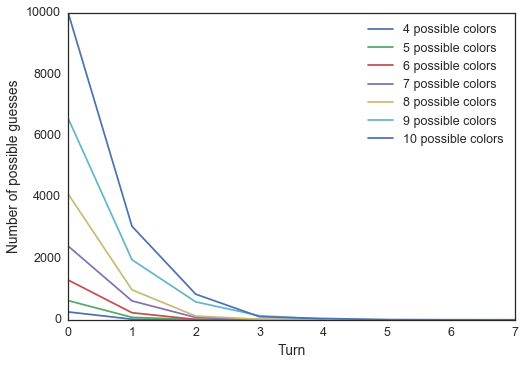
\includegraphics[width=0.6\textwidth]{img/num_guesses}
\caption{Evolution in number of possible guesses}
\label{fig:num_guesses}
\end{figure}

\begin{figure}[!htbp]
\centering
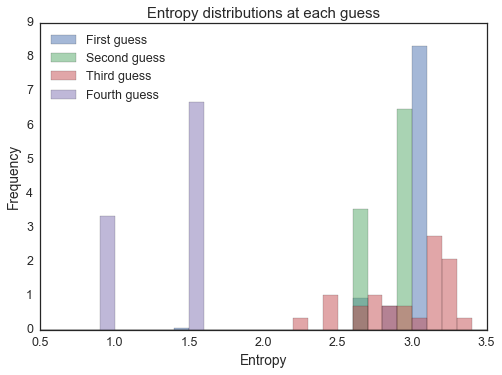
\includegraphics[width=0.6\textwidth]{img/entropy}
\caption{Entropy distributions for classic game parameters}
\label{fig:entropy}
\end{figure}

\newpage
\section{Results by Optimization Method}\label{graphical_results}

\subsection*{Game configuration: 4 positions, varying number of possible colors}

\begin{figure}[h!]
\centering
\subfloat[Number of guesses]{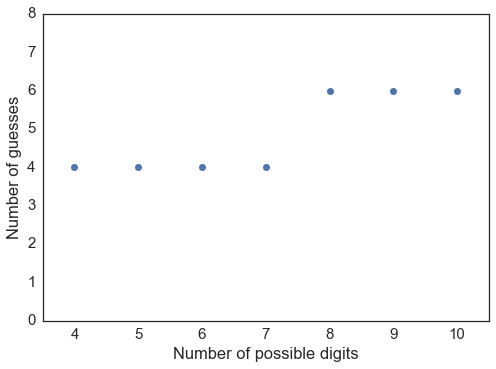
\includegraphics[width=3.4in]{img/knuth_guesses}}
\subfloat[Runtime (seconds)]{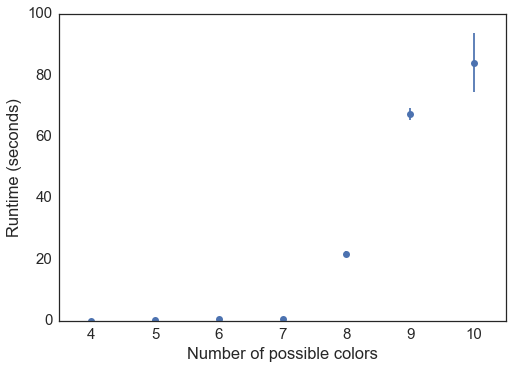
\includegraphics[width=3.4in]{img/knuth_runtime}}
\caption{Knuth's algorithm}
\label{fig:knuth}
\end{figure}

\begin{figure}[h!]
\centering
\subfloat[Number of guesses]{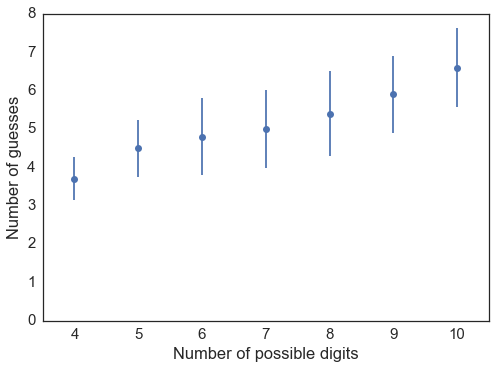
\includegraphics[width=3.4in]{img/randomsearch_guesses}}
\subfloat[Runtime (seconds)]{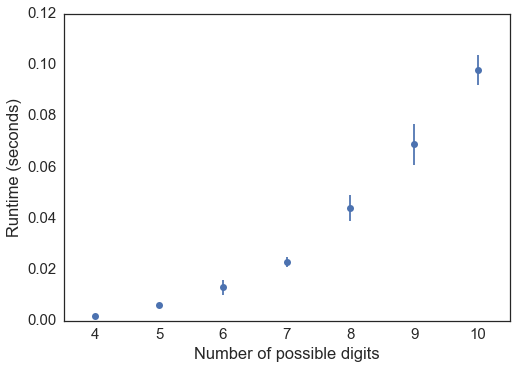
\includegraphics[width=3.4in]{img/randomsearch_runtime}}
\caption{Random search with constraints / Random sampling from posterior}
\label{fig:randomsearch}
\end{figure}

\newpage

\begin{figure}[h!]
\centering
\subfloat[Number of guesses]{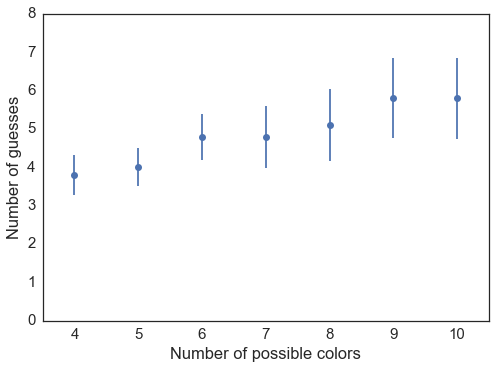
\includegraphics[width=3.4in]{img/entropyall_guesses}}
\subfloat[Runtime (seconds)]{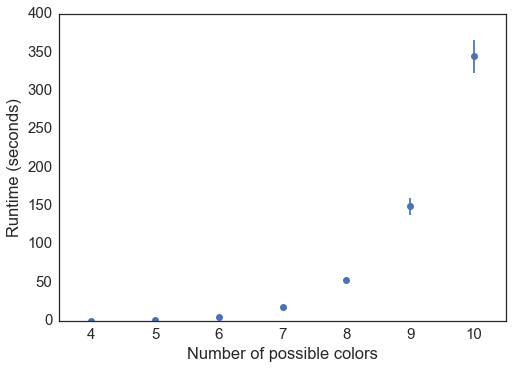
\includegraphics[width=3.4in]{img/entropyall_runtime}}
\caption{Maximizing entropy (all steps)}
\label{fig:entropyall}
\end{figure}

\begin{figure}[h!]
\centering
\subfloat[Number of guesses]{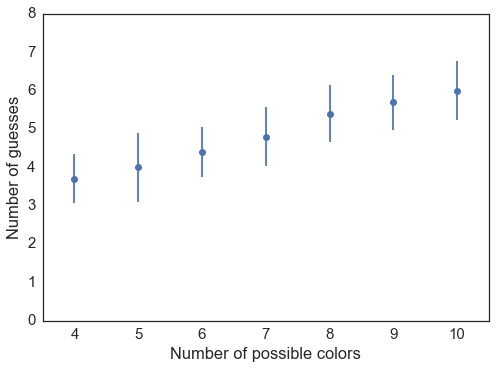
\includegraphics[width=3.4in]{img/entropyminusone_guesses}}
\subfloat[Runtime (seconds)]{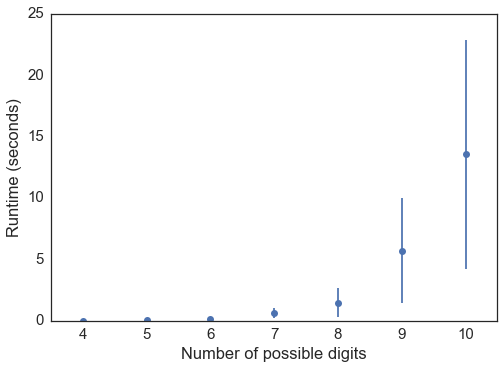
\includegraphics[width=3.4in]{img/entropyminusone_runtime}}
\caption{Maximizing entropy (except first step)}
\label{fig:entropyminusone}
\end{figure}

\newpage

\begin{figure}[h!]
\centering
\subfloat[Number of guesses]{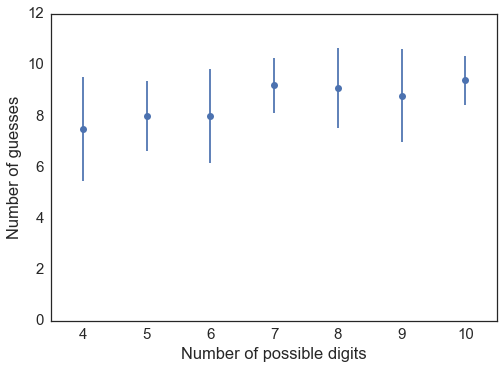
\includegraphics[width=3.4in]{img/sabernier_guesses}}
\subfloat[Runtime (seconds)]{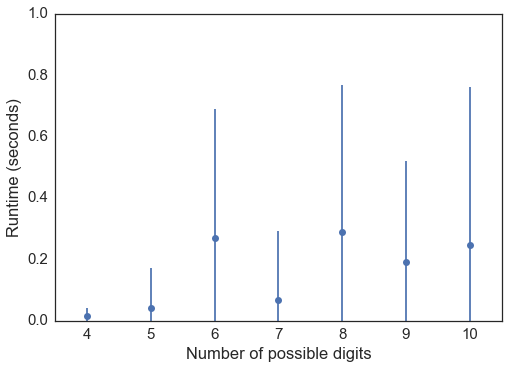
\includegraphics[width=3.4in]{img/sabernier_runtime}}
\caption{Simulated annealing (Bernier objective function)}
\label{fig:sabernier}
\end{figure}

\begin{figure}[h!]
\centering
\subfloat[Number of guesses]{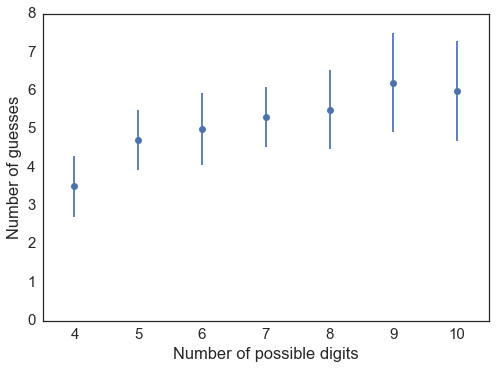
\includegraphics[width=3.4in]{img/saentropy_guesses}}
\subfloat[Runtime (seconds)]{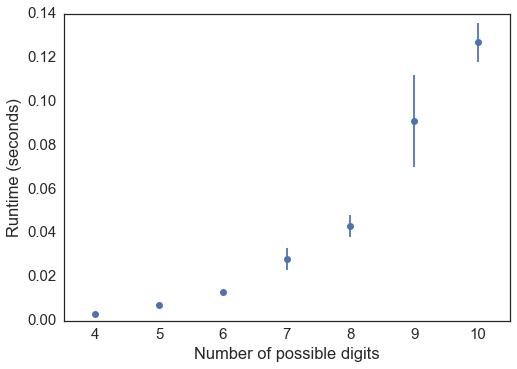
\includegraphics[width=3.4in]{img/saentropy_runtime}}
\caption{Simulated annealing (entropy objective function)}
\label{fig:saentropy}
\end{figure}

\newpage

\begin{figure}[h!]
\centering
\subfloat[Number of guesses]{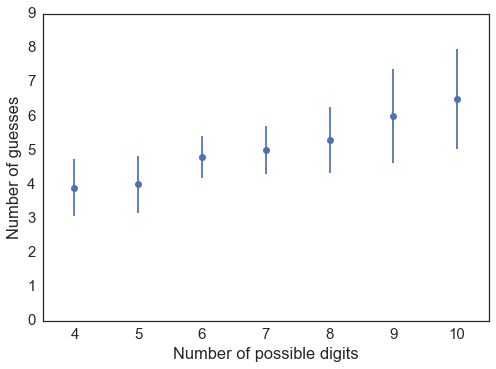
\includegraphics[width=3.4in]{img/gabernier_guesses}}
\subfloat[Runtime (seconds)]{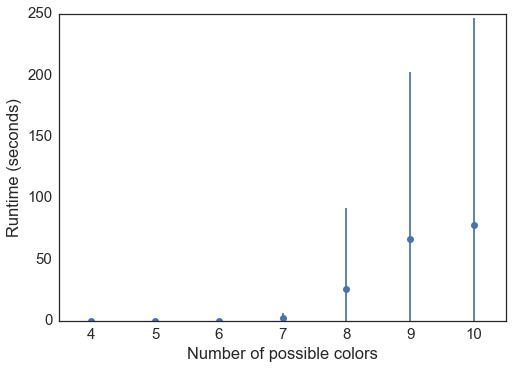
\includegraphics[width=3.4in]{img/gabernier_runtime}}
\caption{Genetic algorithms (Bernier objective function)}
\label{fig:gabernier}
\end{figure}

\begin{figure}[h!]
\centering
\subfloat[Number of guesses]{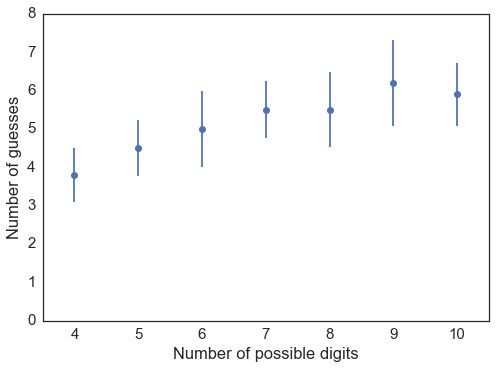
\includegraphics[width=3.4in]{img/gaentropy_guesses}}
\subfloat[Runtime (seconds)]{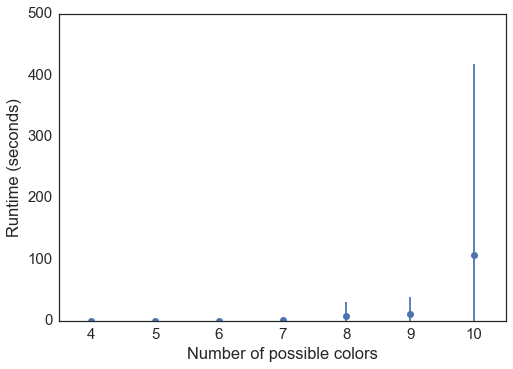
\includegraphics[width=3.4in]{img/gaentropy_runtime}}
\caption{Genetic algorithms (entropy objective function)}
\label{fig:gaentropy}
\end{figure}

\newpage

\subsection*{Game configuration: 2 possible colors, varying number of positions}

\begin{figure}[h!]
\centering
\subfloat[Number of guesses]{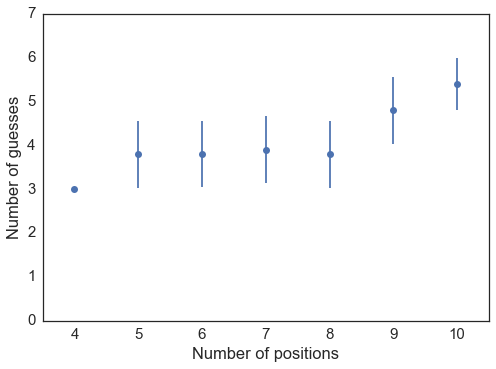
\includegraphics[width=3.4in]{img/knuth_guesses2}}
\subfloat[Runtime (seconds)]{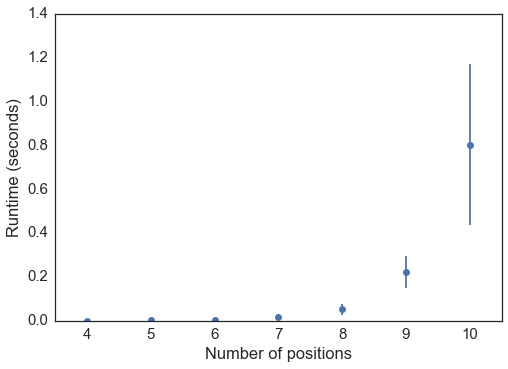
\includegraphics[width=3.4in]{img/knuth_runtime2}}
\caption{Knuth's algorithm}
\label{fig:knuth2}
\end{figure}

\begin{figure}[h!]
\centering
\subfloat[Number of guesses]{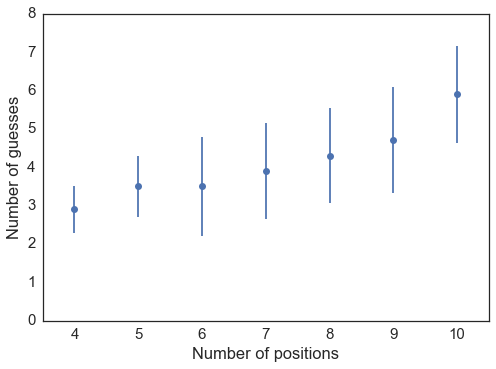
\includegraphics[width=3.4in]{img/randomsearch_guesses2}}
\subfloat[Runtime (seconds)]{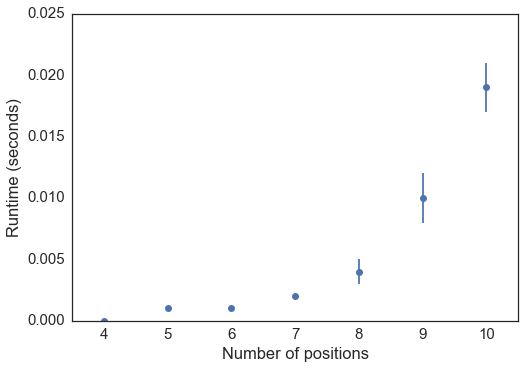
\includegraphics[width=3.4in]{img/randomsearch_runtime2}}
\caption{Random search with constraints / Random sampling from posterior}
\label{fig:randomsearch2}
\end{figure}

\newpage

\begin{figure}[h!]
\centering
\subfloat[Number of guesses]{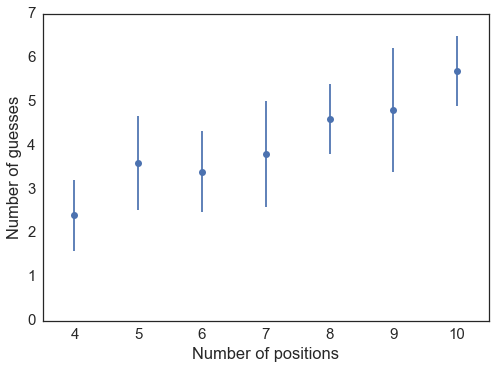
\includegraphics[width=3.4in]{img/entropyall_guesses2}}
\subfloat[Runtime (seconds)]{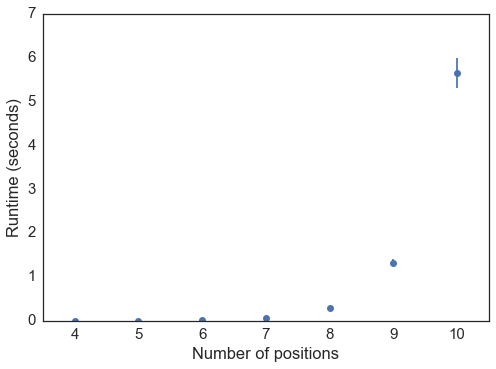
\includegraphics[width=3.4in]{img/entropyall_runtime2}}
\caption{Maximizing entropy (all steps)}
\label{fig:entropyall2}
\end{figure}

\begin{figure}[h!]
\centering
\subfloat[Number of guesses]{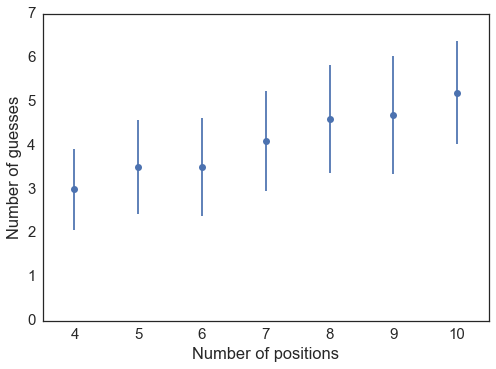
\includegraphics[width=3.4in]{img/entropyminusone_guesses2}}
\subfloat[Runtime (seconds)]{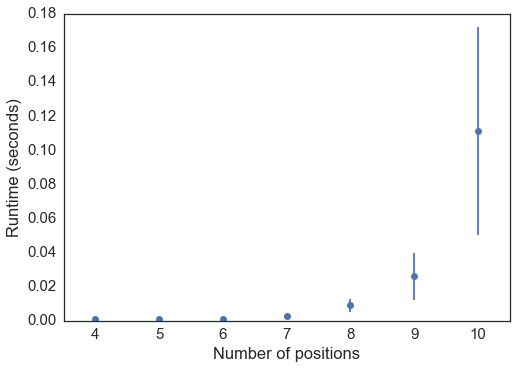
\includegraphics[width=3.4in]{img/entropyminusone_runtime2}}
\caption{Maximizing entropy (except first step)}
\label{fig:entropyminusone2}
\end{figure}

\newpage

\begin{figure}[h!]
\centering
\subfloat[Number of guesses]{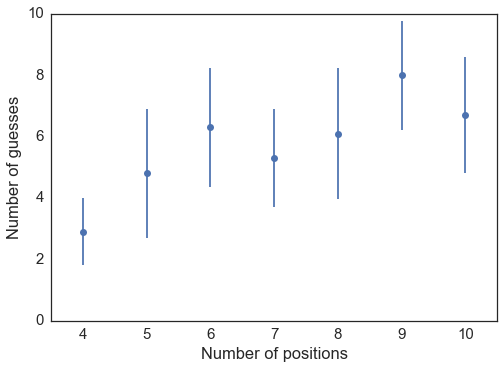
\includegraphics[width=3.4in]{img/sabernier_guesses2}}
\subfloat[Runtime (seconds)]{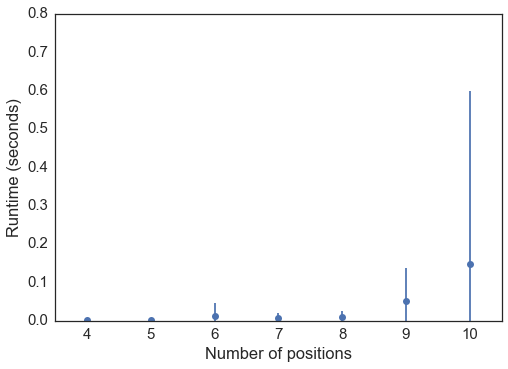
\includegraphics[width=3.4in]{img/sabernier_runtime2}}
\caption{Simulated annealing (Bernier objective function)}
\label{fig:sabernier2}
\end{figure}

\begin{figure}[h!]
\centering
\subfloat[Number of guesses]{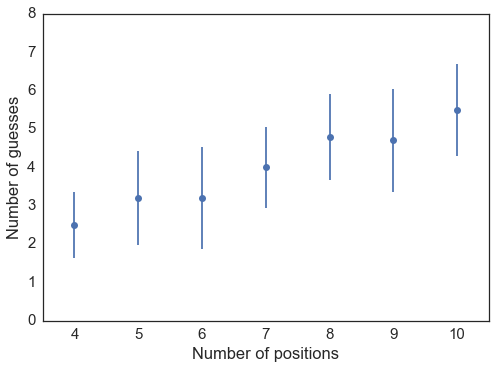
\includegraphics[width=3.4in]{img/saentropy_guesses2}}
\subfloat[Runtime (seconds)]{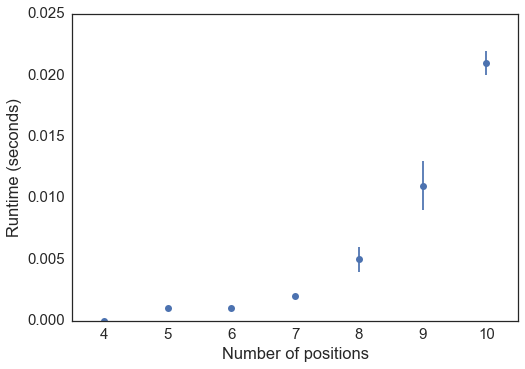
\includegraphics[width=3.4in]{img/saentropy_runtime2}}
\caption{Simulated annealing (entropy objective function)}
\label{fig:saentropy2}
\end{figure}

\newpage

\begin{figure}[h!]
\centering
\subfloat[Number of guesses]{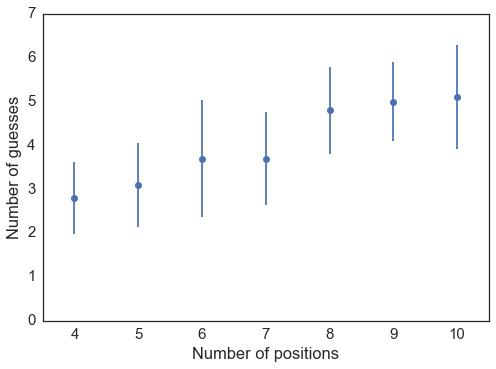
\includegraphics[width=3.4in]{img/gabernier_guesses2}}
\subfloat[Runtime (seconds)]{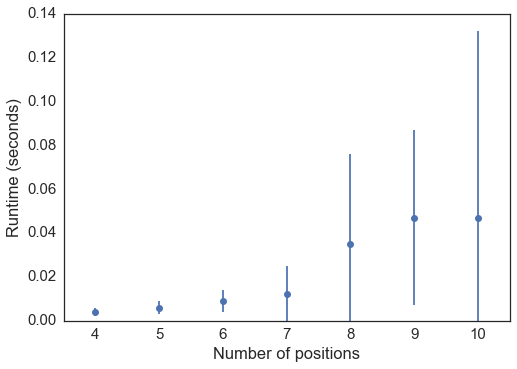
\includegraphics[width=3.4in]{img/gabernier_runtime2}}
\caption{Genetic algorithms (Bernier objective function)}
\label{fig:gabernier2}
\end{figure}

\begin{figure}[h!]
\centering
\subfloat[Number of guesses]{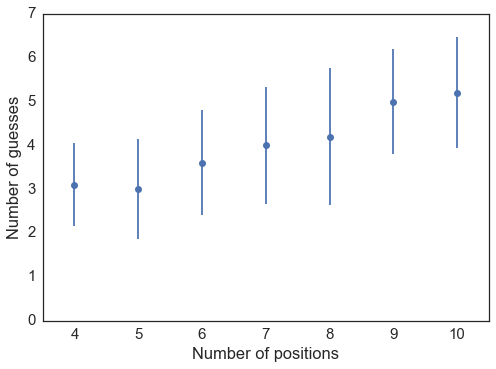
\includegraphics[width=3.4in]{img/gaentropy_guesses2}}
\subfloat[Runtime (seconds)]{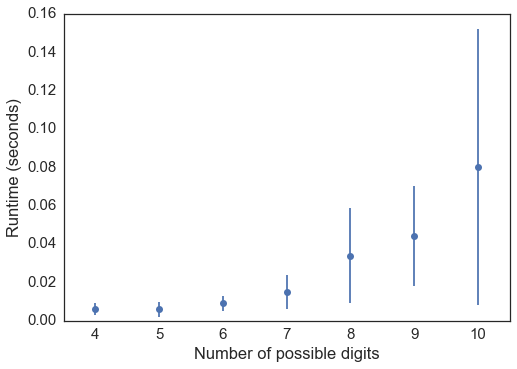
\includegraphics[width=3.4in]{img/gaentropy_runtime2}}
\caption{Genetic algorithms (entropy objective function)}
\label{fig:gaentropy2}
\end{figure}

\newpage
\section{Results by Game Configuration}\label{tabular_results}

\subsection*{Game configuration: 4 positions, varying number of possible colors}

\begin{table}[h!]
\begin{center}
\begin{tabular}{l c c c c}
\toprule
\multirow{2}{*}{\bfseries Optimization method} 		& \multicolumn{2}{c}{\bfseries Number of guesses} 		& \multicolumn{2}{c}{\bfseries Runtime (seconds)}	\\
\cmidrule(lr){2-3}  \cmidrule(lr){4-5}				& $\mu$ & $\sigma$								& $\mu$ & $\sigma$							\\
\cmidrule(lr){1-5}
Knuth's algorithm							& 4.0 & 0.000									& 0.021 & 0.002							\\
Random search / Random sampling				& 3.7 & 0.557									& 0.002 & 0.000							\\
Maximizing entropy (all steps)					& 3.8 & 0.510									& 0.193 & 0.010							\\
Maximizing entropy (except first step)			& 3.7 & 0.640									& 0.007 & 0.004							\\
Simulated annealing (Bernier objective function)	& 7.5 & 2.037									& 0.017 & 0.026							\\
Simulated annealing (entropy objective function)	& 3.5 & 0.805									& 0.003 & 0.001							\\
Genetic algorithms (Bernier objective function)		& 3.9 & 0.831									& 0.022 &	0.026							\\
Genetic algorithms (entropy objective function)		& 3.8 & 0.698									& 0.027 & 0.032							\\
\bottomrule
\end{tabular}
\end{center}
\caption{4 positions; 4 possible colors}
\label{fig:compare_4_4}
\end{table}

\begin{table}[h!]
\begin{center}
\begin{tabular}{l c c c c}
\toprule
\multirow{2}{*}{\bfseries Optimization method} 		& \multicolumn{2}{c}{\bfseries Number of guesses} 		& \multicolumn{2}{c}{\bfseries Runtime (seconds)}	\\
\cmidrule(lr){2-3}  \cmidrule(lr){4-5}				& $\mu$ & $\sigma$								& $\mu$ & $\sigma$							\\
\cmidrule(lr){1-5}
Knuth's algorithm							& 4.0 & 0.000									& 0.264 & 0.006							\\
Random search / Random sampling				& 4.5 & 0.742									& 0.006 & 0.001							\\
Maximizing entropy (all steps)					& 4.0 & 0.497									& 1.147 & 0.035							\\
Maximizing entropy (except first step)			& 4.0 & 0.894									& 0.042 &	0.017							\\
Simulated annealing (Bernier objective function)	& 8.0 & 1.359									& 0.042 & 0.129							\\
Simulated annealing (entropy objective function)	& 4.7 & 0.781									& 0.007 & 0.001							\\
Genetic algorithms (Bernier objective function)		& 4.0 & 0.837									& 0.160 & 0.289							\\
Genetic algorithms (entropy objective function)		& 4.5 & 0.740									& 0.273 & 0.442							\\
\bottomrule
\end{tabular}
\end{center}
\caption{4 positions; 5 possible colors}
\label{fig:compare_4_5}
\end{table}

\newpage

\begin{table}[h!]
\begin{center}
\begin{tabular}{l c c c c}
\toprule
\multirow{2}{*}{\bfseries Optimization method} 		& \multicolumn{2}{c}{\bfseries Number of guesses} 		& \multicolumn{2}{c}{\bfseries Runtime (seconds)}	\\
\cmidrule(lr){2-3}  \cmidrule(lr){4-5}				& $\mu$ & $\sigma$								& $\mu$ & $\sigma$							\\
\cmidrule(lr){1-5}
Knuth's algorithm							& 4.0 & 0.000									& 0.606 & 0.017							\\
Random search / Random sampling				& 4.8 & 0.994									& 0.013 & 0.003							\\
Maximizing entropy (all steps)					& 4.8 & 0.600									& 5.225 & 0.207							\\
Maximizing entropy (except first step)			& 4.4 & 0.663									& 0.145 & 0.099							\\
Simulated annealing (Bernier objective function)	& 8.0 & 1.844									& 0.268 & 0.421							\\
Simulated annealing (entropy objective function)	& 5.0 & 0.949									& 0.013 & 0.001							\\
Genetic algorithms (Bernier objective function)		& 4.8 & 0.622									& 0.230 & 0.472							\\
Genetic algorithms (entropy objective function)		& 5.0 & 1.000									& 0.376 & 0.660 							\\
\bottomrule
\end{tabular}
\end{center}
\caption{4 positions; 6 possible colors}
\label{fig:compare_4_6}
\end{table}

\begin{table}[h!]
\begin{center}
\begin{tabular}{l c c c c}
\toprule
\multirow{2}{*}{\bfseries Optimization method} 		& \multicolumn{2}{c}{\bfseries Number of guesses} 		& \multicolumn{2}{c}{\bfseries Runtime (seconds)}	\\
\cmidrule(lr){2-3}  \cmidrule(lr){4-5}				& $\mu$ & $\sigma$								& $\mu$ & $\sigma$							\\
\cmidrule(lr){1-5}
Knuth's algorithm							& 4.0 & 0.000									& 0.528 & 0.014							\\
Random search / Random sampling				& 5.0 & 1.023									& 0.023 & 0.002							\\
Maximizing entropy (all steps)					& 4.8 & 0.812									& 18.600 & 0.883							\\
Maximizing entropy (except first step)			& 4.8 & 0.766									& 0.669 & 0.407							\\
Simulated annealing (Bernier objective function)	& 9.2 & 1.077									& 0.069 & 0.224							\\
Simulated annealing (entropy objective function)	& 5.3 & 0.781									& 0.028 & 0.005							\\
Genetic algorithms (Bernier objective function)		& 5.0 & 0.707									& 2.432 & 3.576							\\
Genetic algorithms (entropy objective function)		& 5.5 & 0.742									& 1.384 & 2.043							\\
\bottomrule
\end{tabular}
\end{center}
\caption{4 positions; 7 possible colors}
\label{fig:compare_4_7}
\end{table}

\newpage

\begin{table}[h!]
\begin{center}
\begin{tabular}{l c c c c}
\toprule
\multirow{2}{*}{\bfseries Optimization method} 		& \multicolumn{2}{c}{\bfseries Number of guesses} 		& \multicolumn{2}{c}{\bfseries Runtime (seconds)}	\\
\cmidrule(lr){2-3}  \cmidrule(lr){4-5}				& $\mu$ & $\sigma$								& $\mu$ & $\sigma$							\\
\cmidrule(lr){1-5}
Knuth's algorithm							& 6.0 & 0.000									& 21.711 & 0.269							\\
Random search / Random sampling				& 5.4 & 1.114									& 0.044 & 0.005							\\
Maximizing entropy (all steps)					& 5.1 & 0.943									& 53.689 & 1.944							\\
Maximizing entropy (except first step)			& 5.4 & 0.735									& 1.464 & 1.162							\\
Simulated annealing (Bernier objective function)	& 9.1 & 1.578									& 0.290 & 0.478							\\
Simulated annealing (entropy objective function)	& 5.5 & 1.023									& 0.043 & 0.005							\\
Genetic algorithms (Bernier objective function)		& 5.3 & 0.954									& 25.809 & 65.751							\\
Genetic algorithms (entropy objective function)		& 5.5 & 0.973									& 7.866 & 22.396							\\
\bottomrule
\end{tabular}
\end{center}
\caption{4 positions; 8 possible colors}
\label{fig:compare_4_8}
\end{table}

\begin{table}[h!]
\begin{center}
\begin{tabular}{l c c c c}
\toprule
\multirow{2}{*}{\bfseries Optimization method} 		& \multicolumn{2}{c}{\bfseries Number of guesses} 		& \multicolumn{2}{c}{\bfseries Runtime (seconds)}	\\
\cmidrule(lr){2-3}  \cmidrule(lr){4-5}				& $\mu$ & $\sigma$								& $\mu$ & $\sigma$							\\
\cmidrule(lr){1-5}
Knuth's algorithm							& 6.0 & 0.000									& 67.299 & 1.928							\\
Random search / Random sampling				& 5.9 & 0.995									& 0.069 & 0.008							\\
Maximizing entropy (all steps)					& 5.8 & 1.043									& 149.057 & 11.014							\\
Maximizing entropy (except first step)			& 5.7 & 0.714									& 5.702 & 4.282							\\
Simulated annealing (Bernier objective function)	& 8.8 & 1.824									& 0.191 & 0.331							\\
Simulated annealing (entropy objective function)	& 6.2 & 1.288									& 0.091 & 0.021							\\
Genetic algorithms (Bernier objective function)		& 6.0 & 1.378									& 66.406 & 135.881							\\
Genetic algorithms (entropy objective function)		& 6.2 & 1.122									& 10.492 & 28.552							\\
\bottomrule
\end{tabular}
\end{center}
\caption{4 positions; 9 possible colors}
\label{fig:compare_4_9}
\end{table}

\newpage

\begin{table}[h!]
\begin{center}
\begin{tabular}{l c c c c}
\toprule
\multirow{2}{*}{\bfseries Optimization method} 		& \multicolumn{2}{c}{\bfseries Number of guesses} 		& \multicolumn{2}{c}{\bfseries Runtime (seconds)}	\\
\cmidrule(lr){2-3}  \cmidrule(lr){4-5}				& $\mu$ & $\sigma$								& $\mu$ & $\sigma$							\\
\cmidrule(lr){1-5}
Knuth's algorithm							& 6.0 & 0.000									& 84.160 & 9.606							\\
Random search / Random sampling				& 6.6 & 1.020									& 0.098 & 0.006							\\
Maximizing entropy (all steps)					& 5.8 & 1.062									& 344.603 & 21.921							\\
Maximizing entropy (except first step)			& 6.0 & 0.775									& 13.557 & 9.339							\\
Simulated annealing (Bernier objective function)	& 9.4 & 0.970									& 0.248 & 0.513							\\
Simulated annealing (entropy objective function)	& 6.0 & 1.304									& 0.127 & 0.009							\\
Genetic algorithms (Bernier objective function)		& 6.5 & 1.466									& 77.632 & 169.038							\\
Genetic algorithms (entropy objective function)		& 5.9 & 0.831									& 107.604 & 310.685						\\
\bottomrule
\end{tabular}
\end{center}
\caption{4 positions; 10 possible colors}
\label{fig:compare_4_10}
\end{table}

\newpage

\subsection*{Game configuration: 2 possible colors, varying number of positions}

\begin{table}[h!]
\begin{center}
\begin{tabular}{l c c c c}
\toprule
\multirow{2}{*}{\bfseries Optimization method} 		& \multicolumn{2}{c}{\bfseries Number of guesses} 		& \multicolumn{2}{c}{\bfseries Runtime (seconds)}	\\
\cmidrule(lr){2-3}  \cmidrule(lr){4-5}				& $\mu$ & $\sigma$								& $\mu$ & $\sigma$							\\
\cmidrule(lr){1-5}
Knuth's algorithm							& 3.0 & 0.000									& 0.001 & 	0.000							\\
Random search / Random sampling				& 2.9 & 0.624									& 0.000 & 0.000 							\\
Maximizing entropy (all steps)					& 2.4 & 0.800									& 0.001 & 0.000 							\\
Maximizing entropy (except first step)			& 3.0 & 0.921									& 0.001 & 0.000 							\\
Simulated annealing (Bernier objective function)	& 2.9 & 1.091									& 0.001 & 0.001 							\\
Simulated annealing (entropy objective function)	& 2.5 & 0.865									& 0.000 & 0.000 							\\
Genetic algorithms (Bernier objective function)		& 2.8 & 0.812									& 0.004 & 0.002 							\\
Genetic algorithms (entropy objective function)		& 3.1 & 0.943									& 0.006 & 0.003							\\
\bottomrule
\end{tabular}
\end{center}
\caption{2 possible colors; 4 positions}
\label{fig:compare_2_4}
\end{table}

\begin{table}[h!]
\begin{center}
\begin{tabular}{l c c c c}
\toprule
\multirow{2}{*}{\bfseries Optimization method} 		& \multicolumn{2}{c}{\bfseries Number of guesses} 		& \multicolumn{2}{c}{\bfseries Runtime (seconds)}	\\
\cmidrule(lr){2-3}  \cmidrule(lr){4-5}				& $\mu$ & $\sigma$								& $\mu$ & $\sigma$							\\
\cmidrule(lr){1-5}
Knuth's algorithm							& 3.8 & 0.766									& 0.002 & 0.000							\\
Random search / Random sampling				& 3.5 & 0.805									& 0.001 & 0.000							\\
Maximizing entropy (all steps)					& 3.6 & 1.068									& 0.005 & 0.001							\\
Maximizing entropy (except first step)			& 3.5 & 1.072									& 0.001 & 0.000							\\
Simulated annealing (Bernier objective function)	& 4.8 & 2.112									& 0.002 & 0.002							\\
Simulated annealing (entropy objective function)	& 3.2 & 1.220									& 0.001 & 0.000							\\
Genetic algorithms (Bernier objective function)		& 3.1 & 0.963									& 0.006 & 0.003							\\
Genetic algorithms (entropy objective function)		& 3.0 & 1.140									& 0.006 & 0.004							\\
\bottomrule
\end{tabular}
\end{center}
\caption{2 possible colors; 5 positions}
\label{fig:compare_2_5}
\end{table}

\newpage

\begin{table}[h!]
\begin{center}
\begin{tabular}{l c c c c}
\toprule
\multirow{2}{*}{\bfseries Optimization method} 		& \multicolumn{2}{c}{\bfseries Number of guesses} 		& \multicolumn{2}{c}{\bfseries Runtime (seconds)}	\\
\cmidrule(lr){2-3}  \cmidrule(lr){4-5}				& $\mu$ & $\sigma$								& $\mu$ & $\sigma$							\\
\cmidrule(lr){1-5}
Knuth's algorithm							& 3.8 & 0.748									& 0.004 & 0.002							\\
Random search / Random sampling				& 3.5 & 1.284									& 0.001 & 0.000							\\
Maximizing entropy (all steps)					& 3.4 & 0.917									& 0.016 & 0.001							\\
Maximizing entropy (except first step)			& 3.5 & 1.118									& 0.001 & 0.000							\\
Simulated annealing (Bernier objective function)	& 6.3 & 1.931									& 0.013 & 0.033							\\
Simulated annealing (entropy objective function)	& 3.2 & 1.327									& 0.001 & 0.000							\\
Genetic algorithms (Bernier objective function)		& 3.7 & 1.345									& 0.009 & 0.005							\\
Genetic algorithms (entropy objective function)		& 3.6 & 1.200									& 0.009 & 0.004							\\
\bottomrule
\end{tabular}
\end{center}
\caption{2 possible colors; 6 positions}
\label{fig:compare_2_6}
\end{table}

\begin{table}[h!]
\begin{center}
\begin{tabular}{l c c c c}
\toprule
\multirow{2}{*}{\bfseries Optimization method} 		& \multicolumn{2}{c}{\bfseries Number of guesses} 		& \multicolumn{2}{c}{\bfseries Runtime (seconds)}	\\
\cmidrule(lr){2-3}  \cmidrule(lr){4-5}				& $\mu$ & $\sigma$								& $\mu$ & $\sigma$							\\
\cmidrule(lr){1-5}
Knuth's algorithm							& 3.9 & 0.768									& 0.015 & 0.004							\\
Random search / Random sampling				& 3.9 & 1.261									& 0.002 & 0.000							\\
Maximizing entropy (all steps)					& 3.8 & 1.208									& 0.065 & 0.004							\\
Maximizing entropy (except first step)			& 4.1 & 1.136									& 0.003 & 0.001							\\
Simulated annealing (Bernier objective function)	& 5.3 & 1.590									& 0.008 & 0.012							\\
Simulated annealing (entropy objective function)	& 4.0 & 1.049									& 0.002 & 0.000							\\
Genetic algorithms (Bernier objective function)		& 3.7 & 1.054									& 0.012 & 0.013							\\
Genetic algorithms (entropy objective function)		& 4.0 & 1.342									& 0.015 & 0.009							\\
\bottomrule
\end{tabular}
\end{center}
\caption{2 possible colors; 7 positions}
\label{fig:compare_2_7}
\end{table}

\newpage

\begin{table}[h!]
\begin{center}
\begin{tabular}{l c c c c}
\toprule
\multirow{2}{*}{\bfseries Optimization method} 		& \multicolumn{2}{c}{\bfseries Number of guesses} 		& \multicolumn{2}{c}{\bfseries Runtime (seconds)}	\\
\cmidrule(lr){2-3}  \cmidrule(lr){4-5}				& $\mu$ & $\sigma$								& $\mu$ & $\sigma$							\\
\cmidrule(lr){1-5}
Knuth's algorithm							& 3.8 & 0.766									& 0.052 & 0.024							\\
Random search / Random sampling				& 4.3 & 1.236									& 0.004 & 0.001							\\
Maximizing entropy (all steps)					& 4.6 & 0.800									& 0.289 & 0.014							\\
Maximizing entropy (except first step)			& 4.6 & 1.241									& 0.009 & 0.004							\\
Simulated annealing (Bernier objective function)	& 6.1 & 2.142									& 0.010 & 0.015							\\
Simulated annealing (entropy objective function)	& 4.8 & 1.122									& 0.005 & 0.001							\\
Genetic algorithms (Bernier objective function)		& 4.8 & 0.994									& 0.035 & 0.041							\\
Genetic algorithms (entropy objective function)		& 4.2 & 1.568									& 0.034 & 0.025							\\
\bottomrule
\end{tabular}
\end{center}
\caption{2 possible colors; 8 positions}
\label{fig:compare_2_8}
\end{table}

\begin{table}[h!]
\begin{center}
\begin{tabular}{l c c c c}
\toprule
\multirow{2}{*}{\bfseries Optimization method} 		& \multicolumn{2}{c}{\bfseries Number of guesses} 		& \multicolumn{2}{c}{\bfseries Runtime (seconds)}	\\
\cmidrule(lr){2-3}  \cmidrule(lr){4-5}				& $\mu$ & $\sigma$								& $\mu$ & $\sigma$							\\
\cmidrule(lr){1-5}
Knuth's algorithm							& 4.8 & 0.766									& 0.221 & 0.074							\\
Random search / Random sampling				& 4.7 & 1.382									& 0.010 & 0.002							\\
Maximizing entropy (all steps)					& 4.8 & 1.410									& 1.323 & 0.075							\\
Maximizing entropy (except first step)			& 4.7 & 1.345									& 0.026 & 0.014							\\
Simulated annealing (Bernier objective function)	& 8.0 & 1.774									& 0.052 & 0.086							\\
Simulated annealing (entropy objective function)	& 4.7 & 1.345									& 0.011 & 0.002							\\
Genetic algorithms (Bernier objective function)		& 5.0 & 0.894									& 0.047 & 0.040							\\
Genetic algorithms (entropy objective function)		& 5.0 & 1.203									& 0.044 & 0.026							\\
\bottomrule
\end{tabular}
\end{center}
\caption{2 possible colors; 9 positions}
\label{fig:compare_2_9}
\end{table}

\newpage

\begin{table}[h!]
\begin{center}
\begin{tabular}{l c c c c}
\toprule
\multirow{2}{*}{\bfseries Optimization method} 		& \multicolumn{2}{c}{\bfseries Number of guesses} 		& \multicolumn{2}{c}{\bfseries Runtime (seconds)}	\\
\cmidrule(lr){2-3}  \cmidrule(lr){4-5}				& $\mu$ & $\sigma$								& $\mu$ & $\sigma$							\\
\cmidrule(lr){1-5}
Knuth's algorithm							& 5.4 & 0.583									& 0.803 & 0.367							\\
Random search / Random sampling				& 5.9 & 1.261									& 0.019 & 0.002							\\
Maximizing entropy (all steps)					& 5.7 & 0.792									& 5.654 & 0.339							\\
Maximizing entropy (except first step)			& 5.2 & 1.178									& 0.111 & 0.061							\\
Simulated annealing (Bernier objective function)	& 6.7 & 1.878									& 0.147 & 0.453							\\
Simulated annealing (entropy objective function)	& 5.5 & 1.203									& 0.021 & 0.001							\\
Genetic algorithms (Bernier objective function)		& 5.1 & 1.179									& 0.047 & 0.085							\\
Genetic algorithms (entropy objective function)		& 5.2 & 1.260									& 0.080 & 0.072							\\
\bottomrule
\end{tabular}
\end{center}
\caption{2 possible colors; 10 positions}
\label{fig:compare_2_10}
\end{table}

\newpage

%necessary for non-cited references to show up
\nocite{runarsson2010adapting}
\nocite{merelo2010finding}
\nocite{doerr2013playing}
\nocite{merelo2013improving}
\nocite{neuwirth1982some}
\nocite{kooi2005yet}
\nocite{berghman2009efficient}

\bibliographystyle{plain} 
\bibliography{project}

\end{document}
